\subsection{Methoden}

Als erstes war die Umsetzung der Simulation notwendig. Nach Herleitung der Differentialgleichung \sectionautorefname{sec:MNN-sim} haben wir diese zunächst mit dem Eulerverfahren %TODO: spezifizieren
gelöst, und konnten so zumindest visuell die Funktionsweise bestätigen. Doch das Eulerverfahren ist nicht sehr praktikabel, da man zwischen großen Zeitschritten mit kumulativen Ungenauigkeiten und kleinen Zeitschritten mit langer Laufzeit wählen muss. Deshalb haben wir danach die Julia-Bibliothek DifferentialEquations.jl verwendet, welche automatisches Lösen von Differntialgleichungen mit verschiedenen Algorithmen bietet. Wir haben die in der Dokumentation empfohlene Kombination von Tsit5 (basierend of Ch. Tsitouras' Runge-Kutta-Verfahren Verfahren aus 2011 \cite{Tsit5}) mit Rosenbrock23 verwendet, welche ähnliche Ergebnisse zu dem Euler-Verfahren mit sehr geringen Zeitschritten liefert, jedoch gleichzeitig deutlich schneller ist (ca. \SI{60}{\milli\second} vs. ca. \SI{500}{\milli\second} für 100 Sekunden simulieren). %TODO
Diese Kombination haben wir für alle Ergebnisse und Analysen verwendet und werden wir als Tsit5 abkürzen.

Um zu testen, wie gut sich ein MNN mit den verschiedenen Algorithmen optimieren lässt, wird zuerst eine Architektur für die MNNs benötigt.
In diesem Projekt wurde eine bereits vorgeschlagene Struktur verwendet \cite{Lee2022}, damit eine bessere Vergleichbarkeit zu den bereits gefundenen Ergebnissen besteht.
Dabei werden die Neuronen in gleichseitigen Dreiecken angeordnet und verbunden.
Diese Dreiecke werden in einem Gitter zusammengebracht, welches oben und unten fixiert ist.
Die auf das System einwirkenden Kräfte greifen an der linken Seite des MNNs an und die gewünschten Veränderungen finden auf der rechten Seite statt.
Diese Architektur wurde nicht dafür entwickelt, ein reales Szenario, in dem MNNs eingesetzt werden könnten, zu simulieren, sondern dient dazu verschiedene Optimierungsalgorithmen mit einer vereinfachten Problemstellung zu testen und zu verstehen, bevor man sie einsetzt.

Für eine systematische Analyse müssen zusätzlich zu der Architektur der MNNs auch die verschiedenen Verhaltensweisen festgelegt werden.
Dafür nutzen wir zufällig generierte Vektoren für die einwirkenden Kräfte (Kraftvektoren) sowie die gewünschten Positionsänderungen in der letzten Schicht (Zielvektoren).
% Jedes Neuron der letzten Schicht hat dabei ein \SI{50}{\percent} Chance, dass der Zielvektor $\begin{pmatrix} 0 \\ 0 \end{pmatrix}$ ist, es also trotz der einwirkenden Kräfte auf der Stelle bleiben \enquote{soll}.
% Bei den Kraftvektoren hat jedes Neuron der ersten Schicht eine \SI{50}{\percent} Chance, keine einwirkende Kraft zu haben, jedoch gibt es immer mindestens einen Kraftvektor.
Die Kraftvektoren werden während jedem Simulationsschritt auf die entsprechenden Neuronen angewendet, die Zielvektoren legen die Zielpositionen ausgehend von der ursprünglichen Startposition fest. %TODO: Dopplung?

Bei diesem Vorgehen sind unmögliche Kombinationen von Verhaltensweisen möglich, z.B. entgegengesetzte Positionsänderungen bei gleichen einwirkenden Kräften (s. Abb. \ref{fig:impossibletraining} (a)).
Um dies zu verhindern, überprüfen wir beim Generieren mehrerer Verhaltensweisen, dass für ein Neuron der gerade zufällig generierte Kraft- / Zielvektor mit allen anderen Vektoren für dieses Neuron mindestens einen vorgegebene Mindestwinkel bildet. 
Sollte dies nicht zutreffen, wird der Vektor neu erstellt.
Für das Generieren von Verhaltensweisen gibt es so drei Parameter:

\begin{itemize}
    \item Der Mindestwinkel zwischen Vektoren
    \item Die Skalierung der Länge der Kraftvektoren
    \item Die Skalierung der Länge der Zielvektoren
\end{itemize}

\begin{figure}[htb]
    \centering
    \scalebox{0.8}{
    \subfloat[]{
    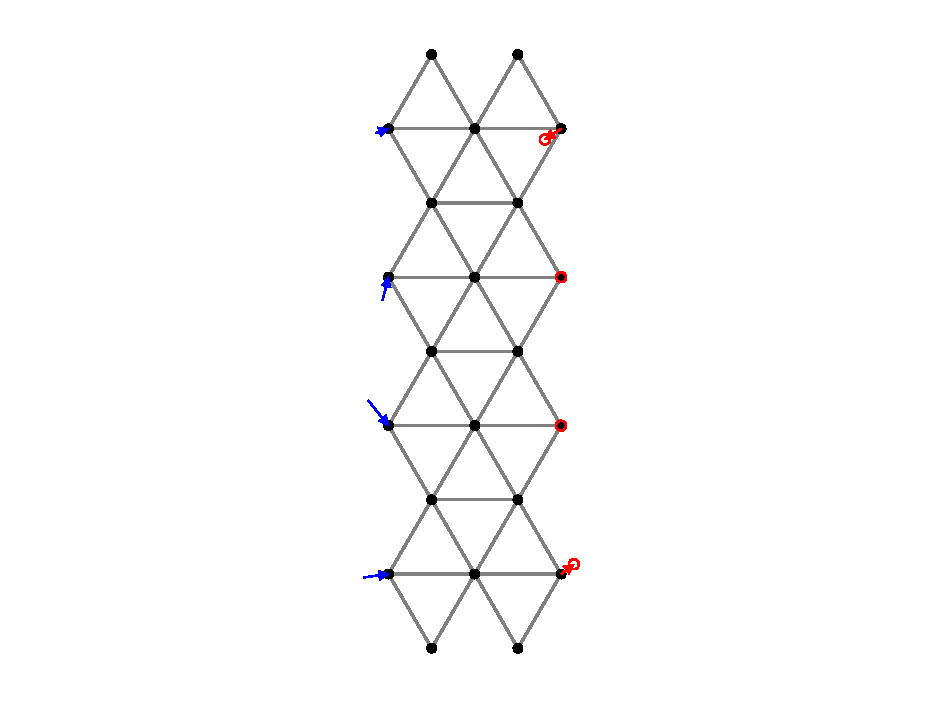
\includegraphics[trim=6cm 0.75cm 6cm 0.75cm, clip]{bilder/impossibleA.pdf}
    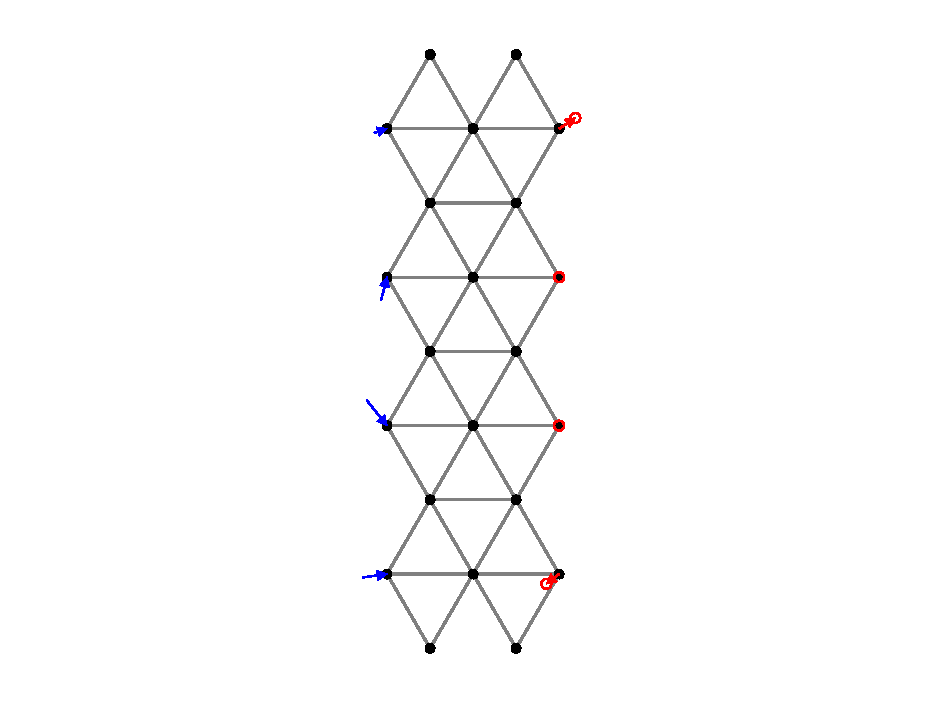
\includegraphics[trim=6cm 0.75cm 6cm 0.75cm, clip]{bilder/impossibleB.pdf}
    }
    \hspace{4em}
    \subfloat[]{
    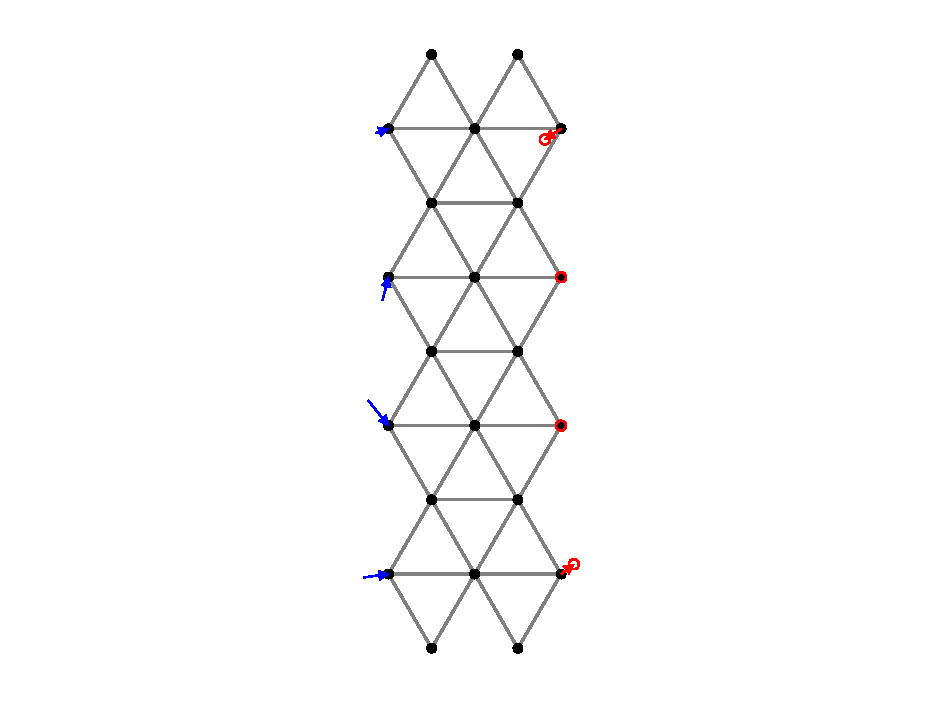
\includegraphics[trim=6cm 0.75cm 6cm 0.75cm, clip]{bilder/impossibleA.pdf}
    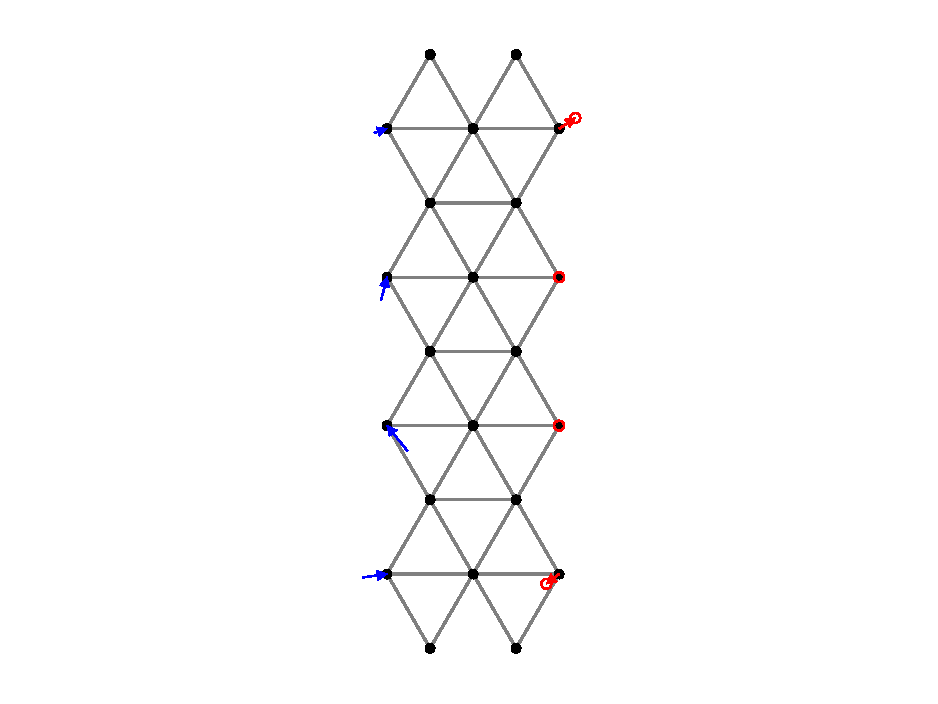
\includegraphics[trim=6cm 0.75cm 6cm 0.75cm, clip]{bilder/impossibleC.pdf}
    }
    }
    \caption{Die schwarzen Punkte sind die Neuronen, die schwarzen Verbindungslinien die Federn. Die obersten und untersten zwei Neuronen sind jeweils fixiert. Die Länge der Kraftvektoren (blau) wurde für bessere Erkennbarkeit verzehnfacht. \\
    \textbf{(a)} Zwei Verhaltensweisen, die gemeinsam unmöglich erfolgreich anzutrainieren sind. Bei beiden sind die Kraftvektoren gleich, die Zielpositionen (rote Kreise) unterscheiden sich jedoch. \\
    \textbf{(b)} Zwei Verhaltensweisen, deren gemeinsames Antrainieren möglich sein könnte, bei uns jedoch nicht vorkommen könnten, da mindestens ein Neuron der ersten Schicht (z.B. erstes von unten) in beiden Verhaltensweisen den gleichen Kraftvektor hat. Somit beträgt der Winkel zwischen diesen \ang{0} und ist entsprechend nie größer als der Mindestwinkel. Im Unterschied zu (a) wurde jedoch der Kraftvektor eines Neurons (rechtes Netzwerk, zweites von unten) verändert.}
    \label{fig:impossibletraining}
\end{figure}

Dieses Vorgehen verhindert zwar unmögliche Szenarien, schließt jedoch auch womöglich schwere, aber nicht unmögliche Kombinationen von Verhaltensweisen aus (s. Abb. \ref{fig:impossibletraining} (b)), 
%TODO: Diskussion?
zu Beginn sollte es jedoch zum Vergleichen der Optimierungsalgorithmen reichen.
% Wenn erfolgreiches Training mit den aktuellen Verhaltensweisen möglich ist, dann werden wir auch schwerer Verhaltensweisen einbringen.

% \begin{figure}
%     \centering
%     \scalebox{0.8}{
%     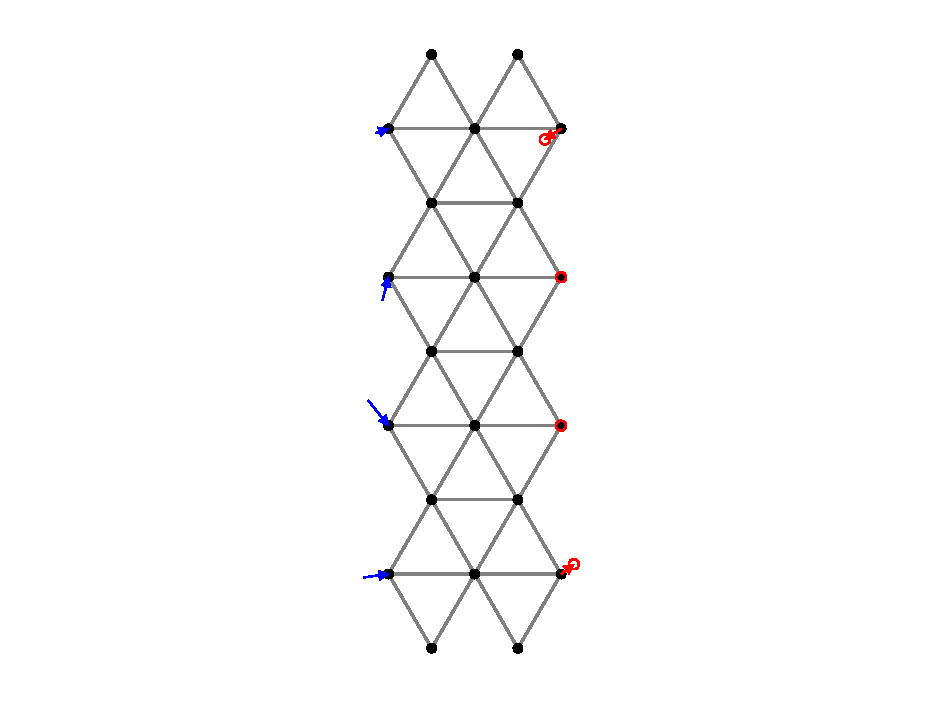
\includegraphics[trim=6cm 0.75cm 6cm 0.75cm, clip]{bilder/impossibleA.pdf}
%     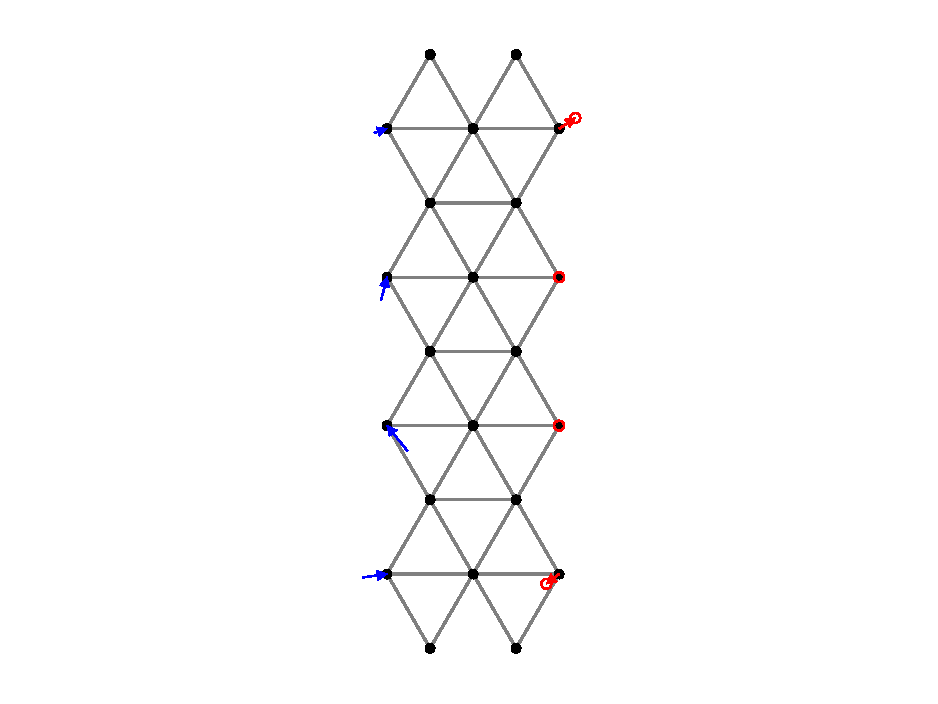
\includegraphics[trim=6cm 0.75cm 6cm 0.75cm, clip]{bilder/impossibleC.pdf}
%     }
%     \caption{Zwei Verhaltensweisen, deren gemeinsames Antrainieren möglich sein könnte, bei uns jedoch nicht vorkommen könnten, da mindestens ein Neuron der ersten Schicht (z.b. erstes von unten) in beiden Verhaltensweisen den gleichen Kraftvektor hat. Somit beträgt der Winkel zwischen diesen \ang{0} und ist entsprechend nie größer als der Mindestwinkel. Im Unterschied zu Abbildung \ref{fig:impossibletraining} wurde jedoch der Kraftvektor eines Neurons (rechtes Netzwerk, zweites von unten) verändert. Die Länge der Kraftvektoren wurde für bessere Erkennbarkeit verzehnfacht.}
%     \label{fig:notimpossibletraining}
% \end{figure}

Der von uns geschriebene Quellcode lässt sich auf höchster Ebene in zwei Teile aufteilen: Unser Paket MNN.jl mit der Implementierung des MNN und der Optimierungsverfahren sowie das Skript Compare.jl für das programmatische Testen und Vergleichen verschiedener Hyperparamerter.
Unter Hyperparameter verstehen wir einen Parameter, welcher nicht Teil des Netzwerks ist (also z.B. keine Federkonstanten), sondern die Struktur sowie das Training dieses Netzwerks beeinflusst (z.B. Optimierungsalgorithmus, Epochen, Mindestwinkel für Verhaltensweisen oder Dimensionen des Netzwerks). 

In Compare.jl verwenden wir CSV.jl zusammen mit DataFrames.jl, um verwendete Hyperparameter sowie den MSE und die Anzahl an bereits trainierten Epochen in CSV-Dateien für spätere Analyse und Vergleiche zu speichern. 
Das Speichern erfolgt dabei alle fünf Epochen.

Mithilfe von Multithreading werden außerdem mehrere Netzwerke gleichzeitig trainiert, teilweise auch mit gleichen Hyperparametern, da ein einzelner Versuch einer Hyperparameterkombination nicht sehr aussagekräftig wäre, v.a. wenn man die Verwendung von Zufallszahlen bei Erstellung von Verhaltensweisen und den Optimierungsalgorithmen bedenkt.

Da so eine Unterscheidung verschiedener Versuche auf Basis anderer Hyperparameter nicht möglich ist, wird jedem neuen Netzwerk eine UUID (\eng{universally unique identifier})
% , erstellt mit der \mintinline{julia}{uuid1()} Funktion der Random.jl-Bibliothek, 
zugeordnet und diese ebenfalls gespeichert.
Andernfalls wäre zum Beispiel das Erstellen des MSE-Verlaufs eines einzelnen Netzwerks über Epochen hinweg nicht möglich.
Diese UUID wird weiter als Startwert für den Zufallszahlengenerator gesetzt, sodass die Versuche reproduzierbar sind.

Insgesamt werden in Compare.jl zum Vergleichen für jedes Netzwerk alle fünf Epochen folgende Daten gespeichert:

\begin{itemize}
    \item aktuelle Zeit
    \item UUID
    \item Gesamtzahl an Trainingsepochen seit Erstellung
    \item Anzahl an Reihen und Spalten des Netzwerks
    \item Anzahl an Verhaltensweisen
    \item oben genannte Parameter für Erstellung der Verhaltensweisen (Mindestwinkel, Skalierungen)
    \item Art der Simulation (Eulerverfahren vs. Tsit5) %TODO: korrekt?
    \item wie viele Sekunden die Simulation jeweils maximal läuft
    \item Mutationsstärke (falls genetischer Algorithmus)
    \item MSE des Netzwerks
\end{itemize}

% \begin{figure}
%     % \centering
%     \filepath{src/}
    
%     \hspace{4em}\filepath{MNN.jl} Hauptpaket, untergeordnete Dateien werden mithilfe von \mintinline{julia}{include(path)} eingefügt 
    
    
%     \caption{Caption}
%     \label{fig:enter-label}
% \end{figure}

Bei den verschieden Testdurchläufen werden immer unterschiedliche Kombinationen von Anzahl der Reihen, Anzahl der Spalten, Anzahl der Verhaltensweisen und den unterschiedlichen Optimierungsalgorithmen festgelegt und der MSE des Netzwerks wird im Verhältnis zur Trainingszeit gespeichert. Mithilfe dieser Daten können nun statistische Analysen durchgeführt werden, um ein besseres Verständnis über die Auswirkungen dieser Eigenschaften zu erlangen.

\subsubsection{Optimierung der Ressonanzkurven}

Wenn man die bereits beschriebenen Ressonanzkurven optimieren möchte ...

\subsubsection{Backpropagation}

Backpropagation ist ein zentrales Konzept in der Funktionsweise von ANNs.
Es handelt sich dabei um einen iterativen Optimierungsalgorithmus, der verwendet wird, um die Gewichtungen der Verbindungen zwischen den Neuronen im Netzwerk anzupassen und somit die Leistung des Netzwerks zu verbessern \cite{brotcrunsher:backwardpass}. Da wir uns in unseren vergangenen Jugend forscht Projekten schon mit ANNs auseinandergesetzt haben, ist uns die Idee gekommen, diesen Algorithmus auch für MNNs umzusetzten.

Der Prozess beginnt mit der Vorwärtspropagation, bei der Eingabedaten durch das Netzwerk fließen und eine Ausgabe erzeugt wird. Der erzeugte Ausgabe-Fehler wird dann durch den Vergleich mit den gewünschten Ausgabewerten berechnet. Im nächsten Schritt wird der Fehler rückwärts durch das Netzwerk propagiert, um die Beiträge jedes Neurons zur Fehlerentstehung zu quantifizieren.
Die Gewichtungen werden entsprechend des Fehlers angepasst, um diesen zu minimieren.

Um diesen Algorithmus für MNNs zu nutzen, benötigt man zum einen eine Möglichkeit, den Fehler durch das Netzwerk zu propagieren, und zum anderen ein Verfahren, das die Federkonstanten anpasst, um den Fehler jedes einzelnen Neurons zu minimieren.
Der Fehler der Neuronen in der letzten Schicht kann einfach mit den Trainingsdaten bestimmt werden. Die Fehler in den Positionen aller anderen Neuronen sind dann der Durchschnitt der Fehler aller Neuronen, mit denen sie verbunden sind. Um herauszufinden, wie wir die Federkonstante einer Feder ändern müssen, damit die Position des Zielneurons einen kleineren Fehler bekommt, muss man erst einmal bestimmen, was der Winkel zwischen dem Fehlervektor und dem Vektor zwischen den beiden Neuronen der Federn ist. Wenn dieser zum Beispiel 90° beträgt, ist eine Änderung der Federkonstante nicht notwendig, da die Kraft den Fehler aufgrund ihrer Richtung nicht beeinflussen kann. Wenn dieser Winkel 0° beträgt, wollen wir die Federkonstante stark erhöhen, da die Kraft der Feder genau mit der Richtung des Fehlers übereinstimmt und wir das Neuron deswegen stärker entlang dieser Richtung bewegen wollen, was durch mehr Kraft erfolgt, wofür wir eine größere Federkonstante benötigen. Wenn der Winkel 180° beträgt, wollen wir die Federkonstante senken, da die Kraft genau in die falsche Richtung ausgeübt wird.

Allgemein wird die Federkonstante also um den folgenden Term erhöht:
{\[
    \frac{\vec{v_1} \cdot \vec{v_2}}{\| \vec{v_1} \| * \| \vec{v_2} \|} * \epsilon
\]}

wobei $v_1$ der Fehler eines Neurons, $v_2$ die Differenz der Positionen der beiden Neuronen einer Feder und $\epsilon$ die Lernrate ist.

Leider ist es uns nicht gelungen, ein MNN mithilfe von Backpropagation zu trainieren, da der MSE nicht signifikant gesunken ist.
Dies könnte zum einen daran liegen, dass Backpropagation voraussetzt, dass die Daten (oder Kräfte) nur in eine Richtung weitergegeben werden können, was bei MNNs nicht der Fall ist.